\chapter{Security in Earnest III \small{\textsf{DRAFT}}}

\section{Recap of last lecture: Security in Earnest (II)}
We proved several bounds in the previous lecture:
\begin{align}
(1-f)pq(n-t) < f &= \Ex[X_r] = 1 - (1-p)^{q(n-t)} < pq(n-t)\label{eq:bound1}\\
\Ex[Y_r] \geq q(n-t)p(1-p)^{q(n-t-1)} &> pq(n-t)(1-pq(n-t)) \geq f(1-f) > \left(1-\frac{\delta}{3}\right)f \label{eq:bound2}\\
(1-\epsilon)\Ex[X(S)] &< X(S) < (1+\epsilon)\Ex[X(S)]\label{eq:bound3}\\
 (1-\epsilon)\Ex[Y(S)] &< Y(S)\label{eq:bound4}\\
Z(S) &< (1+\epsilon)\Ex[Z(S)]\label{eq:bound5}
\end{align}

 First, $X_r$ indicates whether or not round $r$ was successful, i.e. had at least one successful honest query. Bound~\ref{eq:bound1} shows a lower and upper bound for $\E[X_r]$.
 Second, $Y_r$ indicates whether or not round $r$ was a convergence opportunity. Bound~\ref{eq:bound2} gives us a lower bound on $\E[Y_r]$. Bounds~\ref{eq:bound3}, ~\ref{eq:bound4}, and ~\ref{eq:bound5} are Chernoff bounds on $X(S)$, $Y(S)$, and $Z(S)$, respectively where $S$ is a set of consecutive rounds.

 Today, we will be covering Security in Earnest (III). It is highly recommended to read the Bitcoin Backbone paper.

\section{Typicality implies $Z(S) < Y(S)$}
We want to prove that in a typical execution, we have the property that $Z(S) < Y(S)$. This will help us prove that the Common Prefix property holds.

\subsection{Derivation of Upper Bound of $\E[Z(S)]$}
First, we want to derive an upper bound of $\E[Z(S)]$, which will help us achieve our result.
$Z_r$ counts the number of successful queries for the adversary in round $r$. It is a sum of $qt$ repeated independent Bernoulli trials, each with a $p$ chance of succeeding, so $\Ex[Z_r] = pqt$. We can rewrite $pqt$ as $\frac{t}{n-t} pq(n-t)$. Now, if we apply bound~\ref{eq:bound1} we derived from last class and the fact that $\frac{1}{1-f} < 1 + \delta/2$ with $f = \delta/6$ we have that
\begin{align}\Ex[Z_r] &= \frac{t}{n-t} pq(n-t) \\
&< \frac{t}{n-t} \cdot \frac{f}{1-f}\\
&< \left(1 + \frac{\delta}{2}\right)f \frac{t}{n-t}.\label{eq:zexpupper}
\end{align}

% \begin{align*}
%     \Ex[Z_r] &= pqt\\
%      &= \frac{t}{n-t} pq(n-t)\\
%     &< \frac{t}{n-t} \cdot \frac{f}{1-f} \\
%     &< (1 + \delta/2)f \frac{t}{n-t}
% \end{align*}

\subsection{Combining it to get $Z(S) < Y(S)$}
We can use bound~\ref{eq:bound2}, which gives a lower bound on $\E[Y_r]$.
We have that:
\begin{align}
Y(S) & = (1-\epsilon)\Ex[Y(S)] \\
& = (1-\epsilon)\Ex[Y_r] |S| \\
&> (1-\epsilon)f(1-f)|S|\\
&>  \left(1 - \frac{\delta}{3}\right)f|S| \label{eq:ylower}
\end{align}\\
The last inequality is derived as follows by setting $f = \epsilon = \frac{\delta}{6}$:
\begin{align}
 (1-\epsilon)(1-f) &> 1 - \frac{\delta}{3}\\
 \Leftarrow \left(1-\frac{\delta}{6}\right)\left(1-\frac{\delta}{6}\right) &> 1-\frac{\delta}{3}\\
 \Leftarrow \frac{2\delta}{6} + \frac{\delta^2}{36} &> -\frac{\delta}{3}\\
 \Leftarrow \frac{\delta^2}{36} &> 0\\
 \Leftarrow \delta &> 0.
\end{align}
From the Chernoff bound~\ref{eq:bound5} and upper bound~\ref{eq:zexpupper}, we also have that:
\begin{align}
Z(S) &< (1+\epsilon)\Ex[Z(S)]\\
&=(1+\epsilon)\Ex[Z_r]|S|\\
&<(1+\epsilon)\frac{t}{n-t} \cdot \frac{f}{1-f} |S|\\
&<\frac{t}{n-t} \cdot \frac{f}{1-f} |S|+\epsilon\frac{t}{n-t} \cdot \frac{1}{1-f} f|S|\\
&< \frac{t}{n-t} \cdot \frac{f}{1-f} |S| + \epsilon f|S|\label{eq:balance}\\
&\leq \left(1 - \frac{2\delta}{3}\right)f|S|\label{eq:zupper}.
\end{align}\\
To prove inequality~\ref{eq:balance}, note that from the balancing equation we have $f \leq \frac{\delta}{3}$. It suffices to show that $\frac{t}{n-t}\cdot\frac{1}{1-f} < 1$:
\begin{align}
\frac{t}{n-t}\cdot\frac{1}{1-f} &< 1\\
\Leftarrow \frac{1-\delta}{1-f} &< 1\\
\Leftarrow 1-\delta &< 1 -\frac{\delta}{3}.
\end{align}
To prove inequality~\ref{eq:zupper}, we again use our choice of values $f = \epsilon = \frac{\delta}{6}$. Then,
\begin{align}
    \frac{t}{n-t}\cdot\frac{1}{1-f} + \epsilon &< 1 - \frac{2\delta}{3}\\
    \Leftarrow \frac{1-\delta}{1-f} + \epsilon &< 1-\frac{2\delta}{3}\\
    \Leftarrow \frac{1-\delta}{1-\delta/6} + \frac{\delta}{6} &< 1 - \frac{2\delta}{3}\\
    \Leftarrow 1-\delta + \frac{\delta}{6} -\frac{\delta^2}{36} &< 1- \frac{\delta}{6} -\frac{2\delta}{3} + \frac{2\delta^2}{18}\\
    \Leftarrow -\frac{5\delta}{6}-\frac{\delta^2}{36} &< \frac{5\delta}{6} + \frac{\delta^2}{9}\\
    \Leftarrow -\frac{\delta^2}{36} < \frac{\delta^2}{9}
\end{align}
Combining results~\ref{eq:zupper} and~\ref{eq:ylower} together gives us:
\begin{align}
Z(S) < \left(1 - \frac{2\delta}{3}\right)f|S| <  \left(1 - \frac{\delta}{3}\right)f|S| <
Y(S).
\end{align}

\section{Proof of Chain Growth}
% not sure what to call this theorem exactly
Recall chain growth lemma from the previous lecture.
\begin {lemma}[Chain Growth Lemma]
    Suppose that at round $r$, an honest party $P$ has a chain of length $l$. Then by round $r' \geq r$, every honest party has adopted a chain of length at least $l + \sum_{i=r}^{r'-1} X_i$.
\end {lemma}
Now we are equipped with all the necessary tools to prove our first chain virtue.
\begin{theorem}[Chain Growth]
In a typical execution, Chain Growth is attained with $\tau = (1-\epsilon)f, s \geq \lambda$.
\end{theorem}

\begin{proof}
For rounds $S$, such that $|S| \geq \lambda, X(S) > (1-\epsilon)f|S|$ with overwhelming probability. Invoking the growth chain lemma, it is deduced that the chain grows by at least $(1-\epsilon)f\lambda$. Therefore, the chain velocity is $\tau = (1-\epsilon)f$.
\end{proof}


\section{Proof of Common Prefix}
In order for the common prefix property to be violated, the adversary must have had a separate successful query for every convergence opportunity (although, not necessarily during the same round). Any convergence opportunity without a matching adversarial success would lead to convergence among the honest parties. In a nutshell, it must hold that $Z(S) > Y(S)$ over $S$ where $|S|>\lambda$, in order for no convergence to happen.
Our plan for this proof is as follows. We will show this by contradiction. Suppose that CP($k$) is violated. Then,
\begin{enumerate}
    \item We show that it takes a long time to produce these $k$ blocks, so $|S| \geq \lambda$.
    \item We use the pairing lemma: every convergence opportunity is paired to an adverserially successful query, so $Y(S) \leq Z(S)$.
    \item  Lastly, we use our result for typical executions that we can apply as $S$ is large: $Z(S) < Y(S)$, which contradicts the previous point.
\end{enumerate}
The last two points are already proven, so we are only missing the first point to prove Common Prefix.
To do so, we prove the following lemma. We will choose $\lambda$ to be at least $2f$.

\begin{lemma}[Patience Lemma]
In typical executions, any $k \geq 2\lambda f$ blocks have been computed in at least $\frac{k}{2f}$ rounds.
\end{lemma}
\begin{proof}
Let $S'$ be the set of consecutive rounds during which these $k$ blocks were computed. Towards a contradiction, assume that $|S'| < \frac{k}{2f}$. The idea is to apply typicality to the set of rounds $S'$ and to show that, within that small set of rounds, all these $k$ blocks could not possibly have been computed. However, we cannot directly use the set of rounds $S'$, as it is not long enough to apply typicality. We will expand $S'$ to a larger set of rounds $S$ where typicality is applicable, so we need to set $|S| \geq \lambda$. We will do this by including more rounds from the future into $S$. We will then show that, even in this larger $S$, it is impossible that $k$ blocks were computed. So let $S$ be the set of rounds extending $S'$ such that $|S| = \lceil \frac{k}{2f} \rceil + 1 \leq \frac{k}{2f} + 2$. We can now apply typicality to $S$.

The number of blocks that were computed during $S$ is at most $X(S) + Z(S)$ (i.e., they were computed by either the honest parties or the adversary).

We have that
\begin{align}
    X(S) + Z(S) &< (1+\epsilon)\Ex[X(S)] + \left(1 - \frac{2\delta}{3}\right)f|S|\\
    &=(1+\epsilon)f|S|+ \left(1 - \frac{2\delta}{3}\right)f|S|\\
    &= \left(2 + \epsilon - \frac{2\delta}{3}\right)f|S|\\
    &\leq (2-2f)f|S|\label{eq:patiencebal}\\
    & \leq (2-2f)f \cdot \left(\frac{k}{2f} + 2\right)\\
    & = (1-f)(k+4f) \\
    & < k\label{eq:patience-ubound}
\end{align}
The last inequality holds for $k \geq 4$ (this follows from $\lambda \geq 2/f$).
To prove inequality~\ref{eq:patiencebal}, we use the balancing equation $3f + 3\epsilon < \delta$ as follows:
\begin{align}
  2 + \epsilon - \frac{2\delta}{3} &\leq 2-2f\\
  \Leftarrow 3\epsilon - 2\delta &\leq -6f\\
  \Leftarrow 3f + \frac{3}{2}\epsilon &\leq \delta\\
  \Leftarrow 3f + \frac{3}{2}\epsilon &\leq 3f + 3\epsilon
\end{align}
Since we wanted at least $k$ blocks, inequality~\ref{eq:patience-ubound} is a contradiction.
\end{proof}

Recall also the Pairing Lemma from the last lecture.

\begin{lemma}[Pairing Lemma]

Consider a block $C[i]$ produced during a convergence opportunity. If $C'[i] \neq C[i]$, then $C'[i]$ was adversarially computed.
\end{lemma}

We are now ready to prove our second chain virtue.

\begin{theorem}[Common Prefix]
A typical execution satisfies Common Prefix with $k = 2\lambda f$.
\end{theorem}

\begin{figure}
    \centering
    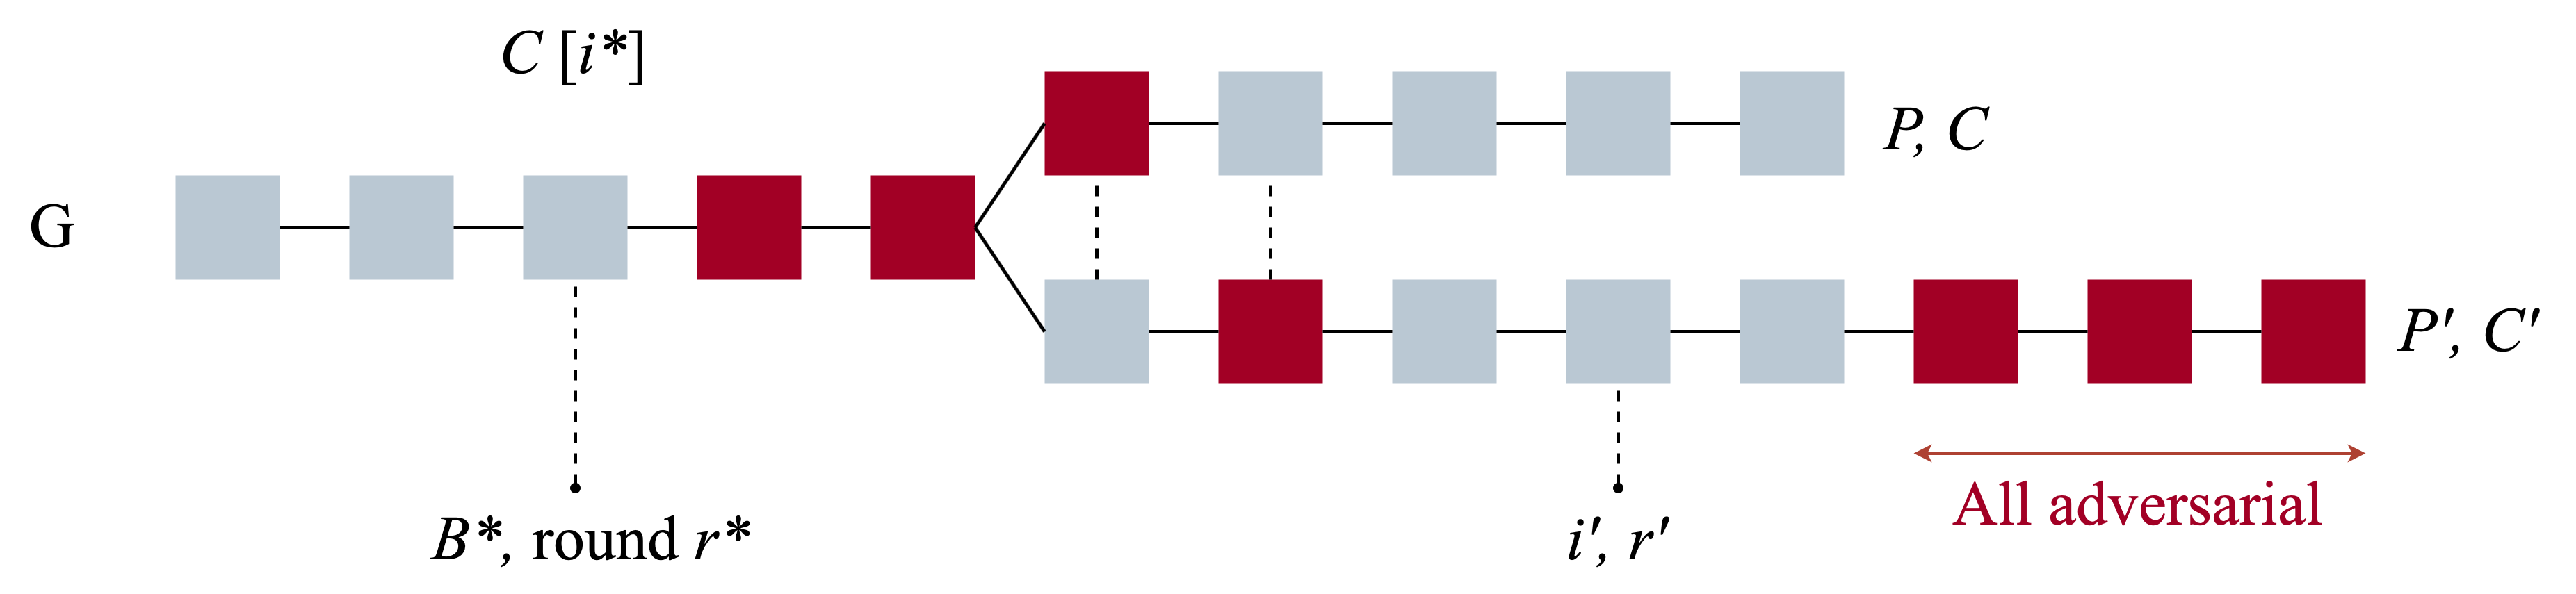
\includegraphics[width=16cm]{figures/common_prefix.png}
    \caption{A common prefix violation. Honestly computed blocks are shown in gray, while adversarially computed blocks are shown in red. At the end of round $r$, party $P$ has adopted chain $C$ and party $P'$ has adopted chain $C'$. $B^\star$ is the most recent honestly produced block in the common prefix of $C,C'$. This is genesis if all other blocks in the common prefix are adversarial. $r'$ is the round with the last convergence opportunity. By the Pairing Lemma, convergence opportunities in rounds after the fork must be matched with a successful adversarial query. For example, $C[i'-3]$ is an adversarially produced block is matched with $C'[i'-3]$, and similarly for $C'[i'-2], C[i'-2]$. It is also possible to have multiple honestly produced blocks in a round after the fork without any convergence opportunities, as $C[i'-1], C'[i'-1]$ show.}
    \label{fig:cp_violation}
\end{figure}

\begin{proof}
Assume towards contradiction that there is a CP$(k)$ violation, illustrated in Figure \ref{fig:cp_violation}.
We have two forks $C, C'$ where if we remove the last $k$ blocks from each of them, they are not the same chain. Let $S = \{ r^*, ..., r\}$, where $r^*$ is the round in which the most recent honestly mined block $C[i^*] = B^*$ in the common prefix of $C, C'$ was produced. After $r^*$, all honest parties will be mining on chains at least $i^*$ long. \\

We claim that $Z(S) \geq Y(S)$. Let $J$ be set of the heights of blocks $B$, where $B$ was produced during a convergence opportunity in $S$. Let $r'$ be the last convergence opportunity in $S$, in which block $B'$ was computed at height $i'$.

We distinguish three cases for the heights of the convergence opportunities within $S$.

Case 1: The blocks between $B^*$ and the fork point are adversarial (by the definition of $r^*$).

Case 2: Any blocks of height larger than $i'$ must be adversarial. To see this, observe that, if there was an honestly produced block with height more than $i'$, then, during round $r'$, the honest party would not have mined at height $i' - 1$. So, all the blocks that exist at height larger than the shorter chain between $C$ and $C'$ must also be adversarial.

Case 3: For the blocks that were produced in the same heights in these two forks, we can apply the Pairing Lemma. We conclude that, since there are two different chains with blocks at this height, one of them must be adversarial.

Thus, overall, we have matched every convergence opportunity with an adversarially successful query. We conclude that $Z(S) \geq Y(S)$.

We have $k$ blocks that were produced in $S$, so by the Patience Lemma, we have $|S| \geq \lambda$, which gives us typicality. However, typicality states that $Z(S) < Y(S)$, a direct contradiction.
\end{proof}




\section{Note about Tradeoffs with $\epsilon$ and $f$}

Let us discuss the relationship between a concrete $\epsilon$ and $\lambda$ obtained by the Chernoff bound.
Larger $\epsilon$ allows for smaller $\lambda$. Let us explore why. The bound on the probability of failure given to us by the Chernoff bound is in the order of $e^{-\epsilon^2 \lambda f}$. Our acceptable probability of failure must be very small and is determined by the security parameter $\kappa$ (recall that typically $\kappa = 256$ and our acceptable probability of failure is $2^{-\kappa}$). Therefore, solving $\kappa = -\epsilon^2 \lambda f$, then we must set $\lambda$ to be large enough to account for the small $\epsilon^2$.

One of the bounds we enforce is:
$$3\epsilon + 3f < \delta$$

Larger $f$ gives larger chain growth since it is easier to produce successful queries. Overall, we want to make both $\epsilon$ and $f$ large, because we like to have quick confirmation (small $\lambda$) and fast chain growth (large $f$). However, we cannot make both of them large, as we are bounded by our honest advantage $\delta$.

The verdict is that, in a setting with a powerful adversary (small $\delta$), we must have a slow chain, either producing blocks slowly, or with the requirement to wait many blocks for confirmation, in order to ensure security. A fast chain with fast confirmation won't cut it.
